\chapter{Numerical Linear Algebra}
\label{ch:numlinalg}

\begin{objectives}
\begin{itemize}
  \item Count the cost of matrix operations and understand why a filter must never form an explicit inverse.
  \item Derive the LU, Cholesky, QR and singular value decompositions, and know which one to use when.
  \item Solve least-squares problems stably, and compute nullspaces, projectors and pseudo-inverses.
  \item Use block matrices, Schur complements and the Woodbury identity fluently.
  \item Understand the matrix exponential, and why the exponential of a skew-symmetric matrix is a rotation.
  \item Understand floating-point arithmetic: rounding, cancellation, conditioning and stability.
\end{itemize}
\end{objectives}

\Cref{ch:linalg} described what matrices \emph{are}. This chapter is about computing with them reliably. A Kalman filter
spends nearly all of its time in a few operations: multiplying matrices, solving linear systems with a covariance matrix,
and factorizing Jacobians. Done naively, these operations are slow, lose accuracy, or silently destroy the symmetry and
positive definiteness of covariances. Done well, they are fast and accurate to nearly machine precision.

% ==============================================================================
\section{The cost of matrix operations}

Numerical analysts count \term{flops} (floating-point operations: one addition or multiplication each). Some basic costs
for $n\times n$ matrices:
\begin{center}\small
\begin{tabular}{@{}l l@{}}
\toprule
Operation & Approximate flops \\
\midrule
dot product of two $n$-vectors & $2n$ \\
matrix-vector product & $2n^2$ \\
matrix-matrix product & $2n^3$ \\
solving a triangular system & $n^2$ \\
LU factorization & $\tfrac23n^3$ \\
Cholesky factorization & $\tfrac13n^3$ \\
explicit inverse & $2n^3$ \\
\bottomrule
\end{tabular}
\end{center}
For the MSCKF with $n = 75$, a matrix product costs about $8\times10^5$ flops, a fraction of a millisecond. Costs grow with the cube of
the dimension, which is why filters keep their state small, exploit block structure, and update only the blocks that change.
We write $\mathcal{O}(n^3)$ (``order $n^3$'') to mean ``at most a constant times $n^3$ for large $n$''.

% ==============================================================================
\section{Triangular systems and the LU factorization}

\subsection{Forward and back substitution}

A triangular system is solved by direct substitution. For an upper-triangular $U$ with non-zero diagonal, the last equation
$U_{nn}x_n = b_n$ gives $x_n$, the previous one then gives $x_{n-1}$, and so on:
\begin{equation}
  x_i = \frac{1}{U_{ii}}\Big(b_i - \sum_{j>i}U_{ij}x_j\Big), \qquad i = n, n-1, \dots, 1 .
\end{equation}
This is \term{back substitution}; \emph{forward substitution} solves lower-triangular systems from the top. Each costs about $n^2$
flops. Every method in this chapter reduces a hard problem to one or two triangular solves.

\subsection{LU factorization}

Gaussian elimination (\cref{sec:linsys}) subtracts multiples $\ell_{ik}$ of row $k$ from the rows below it, column by column, until
the matrix is upper triangular. Recording the multipliers in a unit lower-triangular matrix $L$ gives the \term{LU factorization}
\begin{equation}
  A = LU .
\end{equation}
Then $Ax = b$ is solved by forward substitution $Ly = b$ and back substitution $Ux = y$. The factorization costs $\tfrac23n^3$ flops
once; every additional right-hand side costs only $2n^2$.

\paragraph{Pivoting.} Elimination divides by the pivots. A tiny pivot creates huge multipliers that amplify rounding errors.
The classic example is $\begin{bmatrix}10^{-20} & 1\\ 1 & 1\end{bmatrix}$: eliminating with the pivot $10^{-20}$ gives a multiplier
of $10^{20}$, and in double precision the computed solution of $Ax = (1, 2)$ is completely wrong, although the matrix is
perfectly well conditioned. Swapping the two rows first fixes it. \emph{Partial pivoting} always swaps the row with the largest
available pivot into place, giving $PA = LU$ with a permutation matrix $P$. Symmetric positive-definite matrices, which is
what filters mostly factor, need no pivoting at all, as the next section shows.

% ==============================================================================
\section{The Cholesky factorization}

\begin{theorem}[Cholesky factorization]
\label{thm:cholesky}
\index{Cholesky factorization}
A symmetric matrix $S$ is positive definite if and only if $S = LL\T$ for a lower-triangular $L$ with positive diagonal.
This $L$ is unique.
\end{theorem}
\begin{proof}
If $S = LL\T$ with $L$ invertible, then $x\T Sx = \|L\T x\|^2 > 0$ for $x \ne 0$. Conversely, partition
\begin{equation*}
  S = \begin{bmatrix} s_{11} & s\T \\ s & S_{22} \end{bmatrix}
    = \begin{bmatrix} \ell_{11} & 0 \\ \ell & L_{22} \end{bmatrix}\begin{bmatrix} \ell_{11} & \ell\T \\ 0 & L_{22}\T \end{bmatrix}
    = \begin{bmatrix} \ell_{11}^2 & \ell_{11}\ell\T \\ \ell_{11}\ell & \ell\ell\T + L_{22}L_{22}\T \end{bmatrix}.
\end{equation*}
Matching blocks: $\ell_{11} = \sqrt{s_{11}}$ (positive because $s_{11} = e_1\T Se_1 > 0$), $\ell = s/\ell_{11}$, and
$L_{22}L_{22}\T = S_{22} - ss\T/s_{11}$. The last matrix (a Schur complement, \cref{sec:schur}) is again positive definite, so the
construction continues recursively on a matrix one size smaller. Each step is forced, which proves uniqueness.
\end{proof}

Unrolling the recursion column by column gives the algorithm
\begin{equation}
  L_{jj} = \Big( S_{jj} - \sum_{k<j} L_{jk}^2 \Big)^{1/2}, \qquad
  L_{ij} = \frac{1}{L_{jj}}\Big( S_{ij} - \sum_{k<j} L_{ik}L_{jk} \Big), \quad i > j,
\end{equation}
at a cost of $\tfrac13n^3$ flops, half that of LU. The algorithm is backward stable without pivoting, and it fails (the argument
of a square root is not positive) exactly when $S$ is not numerically positive definite, which makes it a useful diagnostic
too. The variant $S = LDL\T$, with unit-diagonal $L$ and diagonal $D$, avoids square roots; with symmetric pivoting (Eigen's
\code{LDLT}) it also handles semi-definite and slightly indefinite matrices gracefully.

\paragraph{Uses of the Cholesky factor.}
\begin{itemize}
  \item \emph{Solving} $Sx = b$: forward-substitute $Ly = b$, back-substitute $L\T x = y$.
  \item \emph{Whitening}: if a random vector $n$ has covariance $S = LL\T$, then $L\inv n$ has covariance $I$ (\cref{ch:prob}).
        Mahalanobis distances are computed as $r\T S\inv r = \|L\inv r\|^2$ with a single triangular solve.
  \item \emph{Sampling}: if $s$ has covariance $I$, then $Ls$ has covariance $S$.
  \item \emph{Determinants}: $\det S = \prod_iL_{ii}^2$, and $\log\det S = 2\sum_i\log L_{ii}$ without overflow.
\end{itemize}

% ==============================================================================
\section{Orthogonal factorizations: QR}

Orthogonal transformations do not amplify errors (they preserve lengths), so factorizations built from them are the most
stable available.

\subsection{QR from Gram--Schmidt}

Applying Gram--Schmidt to the columns $a_1, \dots, a_n$ of a full-column-rank $A \in \R^{m\times n}$ produces orthonormal $q_1, \dots, q_n$
with $a_k = \sum_{j\le k}r_{jk}q_j$, where $r_{jk} = q_j\T a_k$ and $r_{kk} = \|\tilde q_k\|$. In matrix form
\begin{equation}
  A = Q_1R_1, \qquad Q_1 = [q_1 \cdots q_n] \in \R^{m\times n},\quad Q_1\T Q_1 = I,\quad R_1 \text{ upper triangular}.
\end{equation}
This is the \term{QR factorization}. Classical Gram--Schmidt, implemented literally, loses orthogonality in floating point when the
columns are nearly dependent; the computed $q$'s drift away from being orthogonal. Householder reflections avoid this problem.

\subsection{Householder reflections}

\begin{definition}[Householder reflection]
\index{Householder reflection}
For a non-zero $v \in \R^m$, the matrix $H_v = I - 2\, \dfrac{v v\T}{v\T v}$ reflects vectors across the hyperplane orthogonal to $v$:
it reverses the component along $v$ and leaves the orthogonal components unchanged. It is symmetric and orthogonal, and is its own
inverse: $H_v = H_v\T = H_v\inv$.
\end{definition}

\begin{proposition}[Zeroing a vector below its first entry]
For $x \in \R^m$ not a multiple of $e_1$, let $\alpha = -\operatorname{sign}(x_1)\|x\|$ and $v = x - \alpha e_1$. Then $H_vx = \alpha e_1$.
\end{proposition}
\begin{proof}
Because $\|x\| = \|\alpha e_1\|$, the vectors $x$ and $\alpha e_1$ have the same length, so the reflection across the
perpendicular bisector of the segment joining them swaps them. That bisecting hyperplane is orthogonal to $v = x - \alpha e_1$.
Algebraically: $v\T v = 2\|x\|^2 - 2\alpha x_1$ and $v\T x = \|x\|^2 - \alpha x_1 = \tfrac12v\T v$, so
$H_vx = x - 2v\,\frac{v\T x}{v\T v} = x - v = \alpha e_1$.
\end{proof}

The sign choice makes $v_1 = x_1 + \operatorname{sign}(x_1)\|x\|$ a sum of two numbers of the same sign, avoiding the cancellation
that the other choice would suffer when $x$ is nearly parallel to $e_1$.

\paragraph{Householder QR.} Apply a reflection $H_1$ that zeroes the first column of $A$ below the diagonal; then a reflection $H_2$,
acting on rows $2, \dots, m$, that zeroes the second column below the diagonal; and so on for all $n$ columns:
\begin{equation}
  H_n \cdots H_2 H_1\, A = \begin{bmatrix} R_1 \\ 0 \end{bmatrix}
  \quad\Longleftrightarrow\quad
  A = Q \begin{bmatrix} R_1 \\ 0 \end{bmatrix} = \begin{bmatrix} Q_1 & Q_2 \end{bmatrix}
      \begin{bmatrix} R_1 \\ 0 \end{bmatrix} = Q_1 R_1,
  \label{eq:qr}
\end{equation}
with $Q = H_1 H_2\cdots H_n$ orthogonal ($m\times m$), $R_1 \in \R^{n\times n}$ upper triangular, $Q_1 \in \R^{m\times n}$ and $Q_2 \in \R^{m\times(m-n)}$. The
cost is about $2mn^2 - \tfrac23 n^3$ flops. The form $A = Q[R_1; 0]$ is the \emph{full} QR factorization, and $A = Q_1R_1$ the
\emph{thin} one.

\paragraph{Applying $Q\T$ without forming $Q$.} Each $H_k$ is determined by its vector $v_k$, so $Q\T b = H_n\cdots H_1b$ is computed by
applying the reflections one at a time:
\begin{equation}
  b \;\gets\; b - v_k\,\frac{2\,v_k\T b}{v_k\T v_k}, \qquad k = 1, \dots, n,
\end{equation}
at a cost of $\mathcal{O}(m)$ per reflection. Forming $Q$ explicitly would cost $\mathcal{O}(m^2n)$ flops and $m^2$ storage.

\begin{proposition}[Nullspaces from QR]
\label{prop:qr-nullspace}
If $A$ has full column rank $n$ and $A = Q_1 R_1$ as in \eqref{eq:qr}, then the columns of $Q_1$ are an orthonormal basis of
$\range(A)$ and the columns of $Q_2$ are an orthonormal basis of the left nullspace $\nullsp(A\T)$. In particular $Q_2\T A = 0$.
\end{proposition}
\begin{proof}
$Q\T A = [R_1;\ 0]$, so $Q_2\T A = 0$, i.e.\ the columns of $Q_2$ lie in $\nullsp(A\T)$. They are orthonormal and there are $m - n$ of them,
which is the dimension of $\nullsp(A\T)$ by rank--nullity. Since $R_1$ is invertible, $\range(A) = \range(Q_1)$.
\end{proof}

\begin{implnote}[never form $Q$]
Libraries store the Householder vectors compactly in the lower triangle of the factored matrix. In Eigen,
\code{HouseholderQR::householderQ()} returns a lazy \code{HouseholderSequence} that can be applied to another matrix without
materializing $Q$. This is exactly what the MSCKF needs: it applies the reflections that triangularize a feature Jacobian to the
rest of the measurement equations (\cref{ch:msckfupdate}). Whether a particular call allocates must be checked with the allocation
guard, not assumed.
\end{implnote}

\subsection{Givens rotations}

A \term{Givens rotation} zeroes one entry at a time by rotating a pair of rows. To zero $b$ in the pair $(a, b)$, set
$r = \sqrt{a^2 + b^2}$, $c = a/r$ and $s = b/r$:
\begin{equation}
  \begin{bmatrix} c & s \\ -s & c \end{bmatrix}\begin{bmatrix} a \\ b \end{bmatrix} = \begin{bmatrix} r \\ 0 \end{bmatrix}.
\end{equation}
Embedded in an identity matrix, it acts on two rows of a larger matrix and leaves the others untouched. Givens rotations are
preferred when only a few entries need to be zeroed, when the matrix is sparse, or when rows arrive one at a time. The original
MSCKF paper suggests them for its nullspace projection, because the feature Jacobian has a sparse block structure.

% ==============================================================================
\section{Least squares}
\label{sec:least-squares}

\subsection{The problem and the normal equations}

An overdetermined system $Ax \approx b$, with $A \in \R^{m\times n}$, $m > n$, generally has no exact solution. The \term{least-squares}
solution minimizes the squared residual
\begin{equation}
  f(x) = \|Ax - b\|^2 = x\T A\T Ax - 2x\T A\T b + b\T b .
\end{equation}
Setting the gradient $2A\T Ax - 2A\T b$ to zero gives the \term{normal equations}
\begin{equation}
  A\T A\,x = A\T b .
  \label{eq:normal-equations}
\end{equation}
If $A$ has full column rank, $A\T A$ is positive definite (since $x\T A\T Ax = \|Ax\|^2 > 0$ for $x\ne0$), so the solution is unique and is
a minimum.

\paragraph{Geometric meaning.} The normal equations say $A\T(b - Ax) = 0$: the residual is orthogonal to every column of $A$. The fitted
vector $Ax$ is the orthogonal projection of $b$ onto $\range(A)$, the closest point to $b$ that the model can produce.

\begin{definition}[Orthogonal projector]
\index{projector}
A matrix $\Pi$ is an orthogonal projector if $\Pi^2 = \Pi$ and $\Pi\T = \Pi$. If the columns of $Q$ are an orthonormal basis of a subspace
$\mathcal{S}$, the projector onto $\mathcal{S}$ is $\Pi_{\mathcal{S}} = QQ\T$. For $A$ of full column rank the projector onto $\range(A)$ is
$A(A\T A)\inv A\T$, and $I - \Pi$ projects onto the orthogonal complement.
\end{definition}

Combining the two descriptions of the projector onto $\range(A)$, and recalling that the columns of $Q_2$ in \eqref{eq:qr} span its
complement $\nullsp(A\T)$, gives an identity we will use to prove the optimality of the MSCKF: for any $A_\perp$ whose columns are an
orthonormal basis of the left nullspace of a full-column-rank $H_f$,
\begin{equation}
  A_\perp A_\perp\T = I - H_f (H_f\T H_f)\inv H_f\T .
  \label{eq:nullspace-projector}
\end{equation}

\subsection{Three ways to solve}

\paragraph{Cholesky on the normal equations.} Form $A\T A$ ($mn^2$ flops) and factor it. This is the fastest method, but forming
$A\T A$ squares the condition number of the problem (\cref{sec:conditioning}): $\kappa(A\T A) = \kappa(A)^2$. When $\kappa(A) = 10^8$,
the normal equations lose essentially all sixteen significant digits.

\paragraph{QR.} With $A = Q[R_1; 0]$ and the invariance of lengths under $Q\T$,
\begin{equation}
  \|Ax - b\|^2 = \|Q\T(Ax - b)\|^2 = \|R_1x - Q_1\T b\|^2 + \|Q_2\T b\|^2 .
\end{equation}
The second term does not depend on $x$, and the first vanishes for $x = R_1\inv Q_1\T b$, computed by back substitution. The minimum
residual is $\|Q_2\T b\|$. This method works with the condition number of $A$ itself and is the standard choice.

\paragraph{SVD.} The most robust and most expensive method, required when $A$ may be rank deficient (\cref{sec:svd}).

\subsection{Weighted least squares}

When the equations have different reliabilities, with errors of covariance $W$, the right objective weights each residual by its
uncertainty (\cref{ch:estimation}):
\begin{equation}
  \min_x\ (Ax - b)\T W\inv(Ax - b) .
\end{equation}
With $W = LL\T$ this is ordinary least squares on the \emph{whitened} system $L\inv Ax \approx L\inv b$, and the normal equations become
$A\T W\inv A\,x = A\T W\inv b$.

% ==============================================================================
\section{The singular value decomposition}
\label{sec:svd}

\begin{theorem}[Singular value decomposition]
\label{thm:svd}
\index{singular value decomposition}
Every $A \in \R^{m\times n}$ can be written as $A = U\Sigma V\T$ with $U \in \R^{m\times m}$ and $V \in \R^{n\times n}$ orthogonal and
$\Sigma \in \R^{m\times n}$ diagonal with entries $\sigma_1 \ge \sigma_2 \ge \dots \ge 0$, the \term{singular values}.
\end{theorem}
\begin{proof}[Construction]
$A\T A$ is symmetric and PSD, so by the spectral theorem $A\T A = V\Lambda V\T$ with orthonormal $v_i$ and eigenvalues
$\lambda_1 \ge \dots \ge \lambda_n \ge 0$. Set $\sigma_i = \sqrt{\lambda_i}$. For each $\sigma_i > 0$ define $u_i = Av_i/\sigma_i$. These are
orthonormal: $u_i\T u_j = v_i\T A\T Av_j/(\sigma_i\sigma_j) = \lambda_jv_i\T v_j/(\sigma_i\sigma_j) = \delta_{ij}$. Complete them to an
orthonormal basis $u_1, \dots, u_m$ of $\R^m$. Then $Av_i = \sigma_iu_i$ for all $i$ (for $\sigma_i = 0$, $\|Av_i\|^2 = \lambda_i = 0$),
which in matrix form is $AV = U\Sigma$.
\end{proof}

\begin{figure}[t]
  \centering
  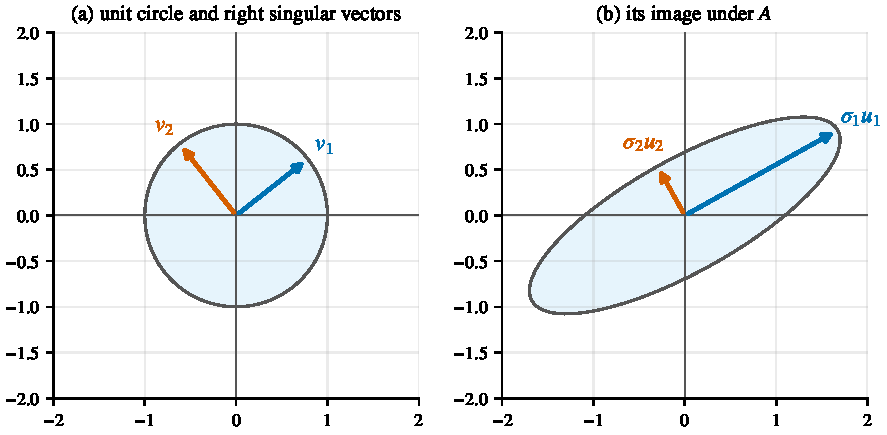
\includegraphics[width=0.9\textwidth]{fig_svd_geometry.pdf}
  \caption{Geometry of the SVD of a $2\times2$ matrix. The right singular vectors $v_1, v_2$ (left) form an orthonormal basis that $A$ maps
  to orthogonal vectors $\sigma_1u_1, \sigma_2u_2$ (right). The unit circle becomes an ellipse with semi-axes $\sigma_1$ and $\sigma_2$: every
  linear map is a rotation, an axis-aligned scaling, and another rotation.}
  \label{fig:svd}
\end{figure}

The SVD says that every linear map, in suitable orthonormal bases of its domain and codomain, is a pure scaling (\cref{fig:svd}). It
reveals everything about $A$ at once:
\begin{itemize}
  \item the rank $r$ is the number of non-zero singular values;
  \item $u_1, \dots, u_r$ span $\range(A)$, $u_{r+1}, \dots, u_m$ span $\nullsp(A\T)$, $v_1, \dots, v_r$ span $\range(A\T)$ and
        $v_{r+1}, \dots, v_n$ span $\nullsp(A)$;
  \item $\|A\|_2 = \sigma_1$ and $\|A\|_F^2 = \sum_i\sigma_i^2$.
\end{itemize}

\paragraph{Pseudo-inverse.} The \term{pseudo-inverse} $A^+ = V\Sigma^+U\T$, where $\Sigma^+$ inverts the non-zero singular values and transposes
the shape, gives the minimum-norm least-squares solution $x = A^+b$ of any system, including rank-deficient ones. For full column
rank, $A^+ = (A\T A)\inv A\T$.

\begin{proposition}[Homogeneous least squares]
\label{prop:homogeneous-ls}
\index{homogeneous least squares}
The unit vector $x$ minimizing $\|Ax\|$ is the right singular vector $v_n$ belonging to the smallest singular value, and the minimum is
$\sigma_n$.
\end{proposition}
\begin{proof}
$\|Ax\|^2 = x\T A\T Ax$, and by the Rayleigh quotient (\cref{prop:rayleigh}) its minimum over unit vectors is the smallest eigenvalue of
$A\T A$, $\sigma_n^2$, attained at the corresponding eigenvector $v_n$.
\end{proof}

Many geometric estimation problems have the form $Ax = 0$ with $x$ known only up to scale: estimating an essential matrix or a homography
from correspondences, or triangulating a point in homogeneous coordinates (\cref{ch:multiview}). With noisy data there is no exact
solution, and \cref{prop:homogeneous-ls} gives the best one.

\begin{theorem}[Best low-rank approximation, Eckart--Young]
\index{Eckart--Young theorem}
Among all matrices of rank at most $k$, the one closest to $A$ in the Frobenius or 2-norm is $A_k = \sum_{i\le k}\sigma_iu_iv_i\T$, obtained by
zeroing all but the $k$ largest singular values.
\end{theorem}

This is how an estimated matrix is projected onto a set defined by its singular values: for example, the nearest valid essential matrix to a
noisy estimate is obtained by replacing its singular values by $(1, 1, 0)$ (\cref{ch:multiview}).

% ==============================================================================
\section{Conditioning and stability}
\label{sec:conditioning}

Two different things can make a computed answer inaccurate: the problem itself may be sensitive to its data, or the algorithm may add more
error than necessary.

\begin{definition}[Condition number]
\index{condition number}
For an invertible (or full-column-rank) $A$, $\kappa(A) = \sigma_{\max}/\sigma_{\min} = \|A\|_2\,\|A^+\|_2$.
\end{definition}

\begin{proposition}[Sensitivity of linear systems]
If $Ax = b$ and $A(x + \delta x) = b + \delta b$, then $\dfrac{\|\delta x\|}{\|x\|} \le \kappa(A)\,\dfrac{\|\delta b\|}{\|b\|}$.
\end{proposition}
\begin{proof}
$\delta x = A\inv\delta b$ gives $\|\delta x\| \le \|A\inv\|\|\delta b\|$, and $b = Ax$ gives $\|b\| \le \|A\|\|x\|$. Multiply the two
inequalities.
\end{proof}

A problem with condition number $\kappa$ can lose about $\log_{10}\kappa$ significant digits whatever the algorithm; it is
\emph{ill-conditioned} when $\kappa$ is large. An algorithm is \emph{backward stable} if its computed answer is the exact answer to a
problem whose data differ from the true data by a few units of rounding error; such an algorithm never loses more than the
conditioning dictates. Householder QR, Cholesky on positive-definite matrices and LU with partial pivoting are backward stable in
practice; classical Gram--Schmidt and the normal equations for ill-conditioned least squares are not. In geometric terms:
triangulating a point seen with almost no parallax is an ill-conditioned problem that no algorithm can rescue
(\cref{ch:multiview}), while recovering the rotation angle from a rotation matrix with $\arccos$ is an unstable algorithm for a
well-conditioned problem (\cref{ch:lie}).

\begin{pitfall}[explicit inverses]
Formulas such as $K = P H\T S\inv$ are notation, not algorithms. Computing $S\inv$ and then multiplying costs about three times as much as
solving, is less accurate, and destroys structure. Factor $S$ once (Cholesky or LDL$^\mathsf{T}$) and solve: $S K\T = H P\T$ gives $K\T$
by two triangular substitutions per column. Writing \code{S.ldlt().solve(Identity)} is still an explicit inverse in disguise.
\end{pitfall}

% ==============================================================================
\section{Block matrices and the Schur complement}
\label{sec:schur}

Estimation constantly partitions vectors and matrices into blocks: IMU state versus clones, poses versus landmarks. Block elimination is
the basic tool.

\begin{proposition}[Block factorization and inverse]
\label{prop:block-inverse}
\index{Schur complement}
Let $M = \begin{bmatrix} A & B \\ C & D \end{bmatrix}$ with $A$ invertible, and define the \term{Schur complement} of $A$ in $M$,
$M/A := D - C A\inv B$. Then
\begin{equation}
  M = \begin{bmatrix} I & 0 \\ C A\inv & I \end{bmatrix}
      \begin{bmatrix} A & 0 \\ 0 & M/A \end{bmatrix}
      \begin{bmatrix} I & A\inv B \\ 0 & I \end{bmatrix},
  \qquad \det M = \det A \cdot \det(M/A),
\end{equation}
and if $M/A$ is invertible,
\begin{equation}
  M\inv = \begin{bmatrix}
    A\inv + A\inv B\, (M/A)\inv\, C A\inv & -A\inv B\, (M/A)\inv \\
    -(M/A)\inv C A\inv & (M/A)\inv
  \end{bmatrix}.
\end{equation}
\end{proposition}
\begin{proof}
Multiply out the three factors. The inverse is the product of the inverses of the three factors in reverse order, and the inverse of a
unit block-triangular factor is obtained by negating its off-diagonal block.
\end{proof}

The Schur complement is what remains of the equations for the second block of unknowns after the first block has been eliminated. To see
this, solve $\begin{bmatrix}A & B\\C & D\end{bmatrix}\begin{bmatrix}x\\y\end{bmatrix} = \begin{bmatrix}f\\g\end{bmatrix}$ by eliminating
$x = A\inv(f - By)$ from the second equation: $(D - CA\inv B)\,y = g - CA\inv f$. For symmetric $M$ with $A \succ 0$, $M \succ 0$ if and only if
$M/A \succ 0$. \Cref{ch:prob} shows that the Schur complement is exactly Gaussian conditioning in covariance form and marginalization in
information form, and \cref{ch:nlls} uses it to eliminate landmarks from bundle adjustment.

\begin{theorem}[Woodbury matrix identity]
\label{thm:woodbury}
\index{Woodbury identity}
For invertible $A$ and $C$ and conformable $U, V$,
\begin{equation}
  (A + U C V)\inv = A\inv - A\inv U \big( C\inv + V A\inv U \big)\inv V A\inv .
\end{equation}
\end{theorem}
\begin{proof}
Write the block matrix $M = \begin{bmatrix} A & U \\ V & -C\inv\end{bmatrix}$ and compute the top-left block of $M\inv$ in two ways with
\cref{prop:block-inverse}. Eliminating $A$ first gives $A\inv + A\inv U(-C\inv - VA\inv U)\inv VA\inv$, the right-hand side. Eliminating the
bottom-right block $-C\inv$ first (the same proposition with the roles of the blocks exchanged) gives the inverse of its Schur complement,
$(A - U(-C\inv)\inv V)\inv = (A + UCV)\inv$.
\end{proof}

Woodbury connects the two forms of the Kalman update (\cref{ch:kf}). It says that a low-rank update of a matrix gives a low-rank update of
its inverse, which is why an update with $m$ measurements needs only an $m\times m$ inverse no matter how large the state is. Its
determinant counterpart is the \emph{matrix determinant lemma} $\det(A + UCV) = \det(C\inv + VA\inv U)\det C\det A$.

% ==============================================================================
\section{The matrix exponential}
\label{sec:matexp}

\begin{definition}[Matrix exponential]
\index{matrix exponential}
For $A \in \R^{n\times n}$, $\exp(A) = \sum_{k=0}^\infty \frac{A^k}{k!} = I + A + \tfrac12 A^2 + \tfrac16 A^3 + \cdots$.
\end{definition}

The series converges for every $A$: the norm of the $k$-th term is at most $\|A\|^k/k!$, and $\sum_k\|A\|^k/k! = e^{\|A\|}$ is finite.

\begin{proposition}[Properties of the matrix exponential]
\label{prop:matexp}
\begin{enumerate}
  \item $\frac{\dd}{\dd t}\exp(tA) = A \exp(tA) = \exp(tA)\, A$.
  \item $x(t) = \exp(tA)\, x_0$ is the unique solution of $\dot x = Ax$, $x(0) = x_0$ (\cref{ch:calculus}).
  \item If $AB = BA$ then $\exp(A + B) = \exp(A)\exp(B)$. \textbf{In general this fails.}
  \item $\exp(A)\inv = \exp(-A)$, and $\exp(A\T) = \exp(A)\T$.
  \item $\exp(T A T\inv) = T \exp(A)\, T\inv$ for invertible $T$.
  \item $\det\exp(A) = e^{\tr A}$.
\end{enumerate}
\end{proposition}
\begin{proof}
(1) Differentiate the series term by term: $\frac{\dd}{\dd t}\frac{t^kA^k}{k!} = A\frac{t^{k-1}A^{k-1}}{(k-1)!}$.
(3) When $A$ and $B$ commute, the binomial theorem holds for $(A + B)^k$, and the Cauchy product of the two series reproduces the series of
$\exp(A + B)$, exactly as for numbers. (4) $A$ and $-A$ commute, so $\exp(A)\exp(-A) = \exp(0) = I$; transposing the series term by term
gives the second statement. (5) $(TAT\inv)^k = TA^kT\inv$. (6) For diagonalizable $A = V\Lambda V\inv$, (5) gives
$\exp(A) = V\exp(\Lambda)V\inv$ with $\exp(\Lambda) = \diag(e^{\lambda_i})$, so $\det\exp(A) = \prod_ie^{\lambda_i} = e^{\sum\lambda_i} = e^{\tr A}$;
the general case follows by continuity, since diagonalizable matrices are dense. Statement (2) is proved in \cref{ch:calculus}.
\end{proof}

The failure of property 3 for non-commuting matrices is the algebraic root of everything subtle about rotations: two rotations generated
by $\sx{a}$ and $\sx{b}$ do not compose into the rotation generated by $\sx{a + b}$. \Cref{ch:lie} measures the discrepancy precisely.

\begin{proposition}[Exponentials of skew-symmetric matrices are rotations]
\label{prop:exp-skew}
If $S\T = -S$ then $\exp(S)$ is a rotation matrix.
\end{proposition}
\begin{proof}
By property 4, $\exp(S)\T\exp(S) = \exp(S\T)\exp(S) = \exp(-S)\exp(S) = I$, so $\exp(S)$ is orthogonal; and
$\det\exp(S) = e^{\tr S} = e^0 = 1$ because a skew-symmetric matrix has a zero diagonal.
\end{proof}

This little proposition is the bridge between the flat world of vectors and the curved world of rotations: every vector $\phi \in \R^3$
defines the rotation $\exp(\sx{\phi})$, and \cref{ch:rotations,ch:lie} show that every rotation arises this way.

\paragraph{Computing the exponential.}
\begin{itemize}
  \item \emph{Nilpotent matrices} ($A^k = 0$ for some $k$): the series is a finite sum.
  \item \emph{Diagonalizable matrices}: $\exp(A) = V\diag(e^{\lambda_i})V\inv$.
  \item \emph{Structured matrices}: when powers of $A$ repeat, as for skew-symmetric $3\times3$ matrices, the series can be summed in closed form
        (Rodrigues' formula, \cref{ch:rotations}).
  \item \emph{General matrices}: \emph{scaling and squaring}. Choose $s$ such that $\|A\|/2^s$ is small, approximate $\exp(A/2^s)$ by a
        truncated series or a rational (Pad\'e) approximation, and square the result $s$ times, using $\exp(A) = \exp(A/2^s)^{2^s}$. This is what
        library routines such as \code{scipy.linalg.expm} do.
\end{itemize}

\begin{example}[Nilpotent generator: the double integrator]
\label{ex:double-integrator}
For $F = \begin{bmatrix} 0 & 1 \\ 0 & 0 \end{bmatrix}$, $F^2 = 0$, so the series terminates:
$\exp(F\Dt) = \begin{bmatrix} 1 & \Dt \\ 0 & 1\end{bmatrix}$. This is the exact transition matrix of position and velocity under zero
acceleration. The inertial error dynamics of \cref{ch:errordyn} have a similar nilpotent structure, so their exponentials can be written in
closed form.
\end{example}

% ==============================================================================
\section{Floating-point arithmetic}
\label{sec:floating}

\subsection{Representation}

\index{floating point}
An IEEE~754 \code{double} represents a number as $\pm1.f\times2^e$, with a sign bit, an 11-bit exponent $e$ and a 52-bit fraction $f$ (53
significant bits counting the implicit leading one). Its range is about $10^{-308}$ to $10^{308}$; results beyond the range \emph{overflow}
to $\pm\infty$, and results below it \emph{underflow} gradually to zero. Undefined operations such as $0/0$ or $\infty - \infty$ produce
\code{NaN} (``not a number''), which propagates through every subsequent operation and compares unequal to everything, including itself.
A single \code{NaN} in a covariance matrix contaminates the whole filter within one update.

\subsection{Rounding}

Two constants describe the precision:
\begin{itemize}
  \item the \term{machine epsilon} $\mach = 2^{-52} \approx 2.22\times10^{-16}$, the gap between $1$ and the next larger double
        (\code{std::numeric\_limits<double>::epsilon()});
  \item the \emph{unit roundoff} $u = 2^{-53} \approx 1.11\times10^{-16}$: every basic operation satisfies
        $\mathrm{fl}(a \circ b) = (a\circ b)(1 + \delta)$ with $|\delta| \le u$.
\end{itemize}
The spacing between consecutive doubles is proportional to their magnitude: near $x$ it is about $\mach|x|$. Relative accuracy is therefore
excellent for a single operation. Errors accumulate in long computations (a sum of $n$ terms can carry a relative error of order $nu$ in the
worst case, though typically $\sqrt n\,u$), but the dramatic losses come from \emph{cancellation}.

\subsection{Cancellation}

Subtracting two nearly equal numbers, each carrying a relative rounding error of size $u$, produces a small result whose \emph{absolute}
error is still of size $u$ times the operands, so its \emph{relative} error can be enormous. The subtraction itself is exact; it merely
exposes the errors already present.

\begin{example}[Catastrophic cancellation in $1 - \cos\theta$]
\label{ex:cancellation}
For $\theta = 10^{-5}$, $\cos\theta = 1 - 5\times10^{-11} + \dots$. The stored value of $\cos\theta$ has an absolute error up to
$u \approx 10^{-16}$, so $1 - \cos\theta \approx 5\times 10^{-11}$ is computed with relative error up to $10^{-16}/(5\times10^{-11}) \approx 2\times
10^{-6}$. Dividing by $\theta^2$ to form $(1-\cos\theta)/\theta^2 \approx 1/2$ keeps that relative error. At $\theta = 10^{-8}$, $\cos\theta$ rounds
to exactly $1$, and the computed value is $0$ instead of $1/2$. The Taylor expansion $\tfrac12 - \tfrac{\theta^2}{24} + \cdots$ has no
cancellation at all. \Cref{fig:taylor} in \cref{ch:lie} shows this effect for all the coefficient functions of the rotation group.
\end{example}

The remedies are always the same: rewrite the expression to avoid the subtraction (for example
$1 - \cos\theta = 2\sin^2(\theta/2)$), use a series expansion in the dangerous regime, or reorganize the algorithm (for example
\code{atan2} instead of \code{acos} for angles, \cref{ch:lie}).

\begin{pitfall}[time stamps in floating point]
EuRoC timestamps are nanoseconds since the Unix epoch, about $1.4\times10^{18}$, which lies between $2^{60}$ and $2^{61}$. A \code{double} near
that value can only represent multiples of $2^{60-52} = 256$~ns. Converting absolute timestamps to \code{double} therefore quantizes them to
256~ns, and accumulating time by repeated addition of $\Dt$ drifts further. Keep absolute time in 64-bit integers
(\code{std::chrono::nanoseconds}) and convert only differences to \code{double} (AGENTS.md C5).
\end{pitfall}

\begin{takeaways}
\begin{itemize}
  \item Costs grow as $n^3$; exploit structure and update only what changes.
  \item Cholesky ($S = LL\T$) is the factorization of choice for covariances: half the cost of LU, stable without pivoting, and a built-in test
        of positive definiteness.
  \item Householder QR is the stable way to solve least squares and to obtain orthonormal bases of a column space and of its complement,
        the left nullspace. Apply $Q\T$ through its reflections; never form $Q$.
  \item The SVD reveals rank, nullspaces and conditioning, and solves homogeneous least squares $\min\|Ax\|$, $\|x\| = 1$.
  \item Schur complements eliminate variables; Woodbury converts between large and small inverses.
  \item $\exp(A + B) \neq \exp(A)\exp(B)$ unless $A$ and $B$ commute; the exponential of a skew-symmetric matrix is a rotation.
  \item Cancellation, not single operations, destroys floating-point accuracy. Time stamps belong in 64-bit integers.
\end{itemize}
\end{takeaways}

\begin{exercises}
  \item Solve $\begin{bmatrix}10^{-20} & 1\\ 1 & 1\end{bmatrix}x = \begin{bmatrix}1\\2\end{bmatrix}$ in double precision by elimination without
        pivoting and with partial pivoting. Explain the difference.
  \item Compute the Cholesky factor of $\begin{bmatrix}4 & 2 & 2\\ 2 & 5 & 3\\ 2 & 3 & 6\end{bmatrix}$ by hand and use it to solve $Sx = (8, 10, 11)$.
  \item Show that if $P\succ0$ then $P - K S K\T \succeq 0$ for $S = HPH\T + R$, $K = PH\T S\inv$ and $R \succ 0$. (Hint: the Schur complement of
        $\begin{bmatrix}S & HP\\ PH\T & P\end{bmatrix}$.)
  \item Implement Householder QR in Python for a $10\times3$ matrix, check \cref{prop:qr-nullspace} numerically, and compare the accuracy of solving
        a least-squares problem with $\kappa(A) = 10^8$ by the normal equations and by QR.
  \item Prove \eqref{eq:nullspace-projector} using a full QR factorization of $H_f$.
  \item Use \cref{thm:woodbury} to show that $\big(P\inv + H\T R\inv H\big)\inv = P - PH\T(HPH\T + R)\inv HP$. Which side is cheaper to evaluate when
        $P$ is $75\times75$ and $R$ is $2\times2$? When $R$ is $500\times500$?
  \item Compute $\exp\big(\begin{bmatrix}0 & -\theta\\ \theta & 0\end{bmatrix}\big)$ by summing the series, and recognize the result.
  \item Show that for $A = \begin{bmatrix}0 & 1\\0 & 0\end{bmatrix}$ and $B = \begin{bmatrix}0 & 0\\1 & 0\end{bmatrix}$,
        $\exp(A + B) \ne \exp(A)\exp(B)$.
  \item What is the spacing of doubles near $2^{30}$ seconds expressed in nanoseconds? Would storing time as \code{double} seconds since the epoch
        be acceptable for a 200~Hz IMU?
  \item Rewrite $\sqrt{x^2 + 1} - x$ for large $x$ and $(1 - \cos x)/x^2$ for small $x$ so that they are computed accurately.
\end{exercises}
